\documentclass[11pt]{article}
\usepackage[margin=1.05in]{geometry}
\usepackage{amsmath,amssymb,amsthm,mathtools,microtype,enumitem}
\usepackage{tikz}
\usepackage[colorlinks=true,linkcolor=blue,citecolor=blue,urlcolor=blue]{hyperref}
\hypersetup{pdftitle={Expected amenable subalgebras preserving core commutants},
  pdfauthor={OpenAI},pdfsubject={The relative bicentralizer conjecture}}
\pdfgentounicode=1
\pdfglyphtounicode{parenleftbig}{0028}
\pdfglyphtounicode{parenleftBigg}{0028}
\pdfglyphtounicode{parenrightbig}{0029}
\pdfglyphtounicode{parenrightBigg}{0029}
\pdfglyphtounicode{angbracketleftBigg}{27E8}
\pdfglyphtounicode{angbracketrightBigg}{27E9}
\pdfglyphtounicode{circlemultiplydisplay}{2A02}
\pdfglyphtounicode{circlemultiplytext}{2A02}
\pdfglyphtounicode{summationtext}{2211}
\pdfglyphtounicode{summationdisplay}{2211}
\pdfglyphtounicode{producttext}{220F}
\pdfglyphtounicode{productdisplay}{220F}
\pdfglyphtounicode{integraltext}{222B}
\pdfglyphtounicode{integraldisplay}{222B}
\pdfglyphtounicode{hatwide}{02C6}
\pdfglyphtounicode{parenlefttp}{239B}
\pdfglyphtounicode{parenleftbt}{239D}
\pdfglyphtounicode{parenrighttp}{239E}
\pdfglyphtounicode{parenrightbt}{23A0}
\pdfglyphtounicode{mapsto}{007C}
\let\originalmapsto\mapsto
\renewcommand{\mapsto}{\mathrel{\pdfliteral direct{/Span << /ActualText <FEFF21A6> >> BDC}\originalmapsto\pdfliteral direct{EMC}}}
\let\originallongmapsto\longmapsto
\renewcommand{\longmapsto}{\mathrel{\pdfliteral direct{/Span << /ActualText <FEFF27FC> >> BDC}\originallongmapsto\pdfliteral direct{EMC}}}
\pdfinfoomitdate=1
\pdftrailerid{}
\pdfsuppressptexinfo=15
\setlength{\emergencystretch}{2em}
\setlist{itemsep=3pt,topsep=5pt}
\newtheorem{theorem}{Theorem}[section]
\newtheorem{proposition}[theorem]{Proposition}
\newtheorem{lemma}[theorem]{Lemma}
\newtheorem{corollary}[theorem]{Corollary}
\theoremstyle{definition}
\newtheorem{remark}[theorem]{Remark}
\DeclareMathOperator{\Ad}{Ad}
\DeclareMathOperator{\supp}{supp}
\DeclareMathOperator{\conv}{conv}
\newcommand{\B}{\mathrm B}
\newcommand{\cM}{c(M)}
\newcommand{\C}{\mathbb C}
\newcommand{\R}{\mathbb R}
\newcommand{\E}{\mathbb E}
\newcommand{\HH}{\mathcal H}
\newcommand{\U}{\mathcal U}
\newcommand{\one}{\mathbf1}
\title{Expected amenable subalgebras\\preserving core commutants}
\author{OpenAI}
\date{September 23, 2026}
\begin{document}
\maketitle
\begin{abstract}
We prove that every inclusion $N\subset M$ of von Neumann algebras with
separable preduals and a faithful normal conditional expectation contains
an expected amenable subalgebra $P\subset N$ such that
$P'\cap c(M)=N'\cap c(M)$, where $c(M)$ denotes the continuous core of $M$.
This resolves the relative bicentralizer conjecture in this setting.
\end{abstract}

\section{Introduction}
An inclusion $N\subset M$ is \emph{expected} if it admits a faithful normal
conditional expectation $E_N:M\to N$. Such an expectation makes the
inclusion compatible with modular theory: a faithful normal state on $N$
extends through $E_N$ to a state on $M$ whose modular action preserves $N$.
For a faithful normal state $\psi$ on $M$, the continuous core is
$c(M)=M\rtimes_{\sigma^\psi}\R$, with its canonical copy of $M$.

We ask whether an amenable expected subalgebra of $N$ can impose exactly
the same commutation constraints as $N$ on the whole core. Equality of
commutants inside $M$ alone does not answer this question: the core also
contains the unitaries implementing the modular action. Our main theorem
retains these additional constraints.

\begin{theorem}\label{thm:main}
Let $N\subset M$ be a unital inclusion of von Neumann algebras with separable
preduals, and suppose that there is a faithful normal conditional expectation
$E_N:M\to N$. There exist a unital amenable von Neumann subalgebra $P\subset N$
and a faithful normal conditional expectation $F:N\to P$ such that
\[
 P'\cap c(M)=N'\cap c(M).
\]
Here amenable means injective.
\end{theorem}
The canonical core isomorphism associated with a change of faithful normal
state fixes $M$, so the stated relative-commutant equality is independent
of the state used to define the core.

\paragraph{History and the relative conjecture.}
Popa's solution of Kadison's problem for irreducible expected inclusions
with separable preduals and type II bottom factor provides
a model for finding amenable subalgebras that retain prescribed
commutation properties \cite{Popa1981}. For type III factors, modular
asymptotic centralization supplies a related approach. The bicentralizer
of a faithful normal state consists of those elements that commute
asymptotically with every bounded sequence asymptotically centralizing
the state in predual norm. Connes introduced the problem of its triviality
in the classification of injective factors \cite{Connes1982,Connes1985}.
Haagerup solved the amenable type $\mathrm{III}_1$ case, completing the
uniqueness theorem for the injective type $\mathrm{III}_1$ factor
\cite{Haagerup}. For type $\mathrm{III}_1$ factors with separable predual,
he characterized
triviality by norm-density of faithful normal states whose centralizers
have trivial relative commutant \cite[Theorem~3.1]{Haagerup}.
His proof uses Popa's construction to find a maximal abelian subalgebra
of such a centralizer that remains maximal abelian in the ambient factor;
the expectations onto the centralizer and onto its abelian subalgebra
compose \cite[proof of Theorem~3.1]{Haagerup}.

Masuda introduced a relative bicentralizer in the finite-index setting
\cite[Definition~4.1]{Masuda2005}.
Ando, Haagerup, Houdayer, and Marrakchi constructed the canonical relative
bicentralizer flow for expected inclusions with type $\mathrm{III}_1$
bottom factor \cite[Theorem~A]{AHHM}. This extends the absolute flow
discovered by Haagerup and independently by Marrakchi, as described in
that paper. The structural results of Houdayer and Isono
\cite[Proposition~3.4 and Theorem~3.5]{HI2017} and Marrakchi's absolute
flow-ergodicity theorem \cite[Theorem~D]{M0} underlie the absolute
reduction used here.
Marrakchi formulated the relative bicentralizer conjecture and proved
that, for separable preduals, it is equivalent to the conclusion of
Theorem~\ref{thm:main} \cite[Conjecture~C and Theorem~D]{M1}.
Our theorem therefore resolves that conjecture positively, including
inclusions with arbitrary centers and types.

Marrakchi's recent Theorem B \cite{M2} gives an expected amenable
subalgebra $P\subset N$ preserving $N'\cap M$ for general expected
inclusions with separable preduals. Theorem~\ref{thm:main} preserves
the commutant in the continuous core. Applying the earlier result with
upper algebra $c(M)$ would require an expectation from $c(M)$ onto $N$,
which the original inclusion does not supply.
The binormal-state and zero-shift completely positive map of
\cite[Lemmas~2.1 and 2.2(1)]{M2} are essential inputs to the proof below.

\paragraph{The absolute problem and the recent announcement.}
Houdayer and Marrakchi have announced that every type $\mathrm{III}_1$
factor admitting a faithful normal state has trivial bicentralizer
\cite[Theorem~G]{HoudayerMarrakchi2026}; their theorem statement has no
separability restriction. Section~\ref{sec:absolute} gives an alternative
proof of its separable-predual instance as part of our relative argument.
The multiplication maps and spectral resonance of
\cite[Section~8]{HoudayerMarrakchi2026} are closely related to this
absolute comparison. Their paper also develops relative bicentralizer
theory for tracial group actions; the general expected-inclusion
core-commutant conclusion of Theorem~\ref{thm:main} is obtained here
through the relative tensor and core argument.

The companion \cite[Theorem~4.1 and Section~5.1]{BoundedRecovery}
develops a complementary absolute argument through bounded recovery:
for a state with scalar centralizer, a fixed multiplication defect whose
modularly averaged squared norm has positive limsup along unit vectors
with spectral supports shrinking to one point can be detected by uniformly
bounded algebra elements.
The binormal-state identity used here also admits the iteration that
yields the relative estimate uniformly in tensor length and flow shifts.

\paragraph{An abelian consequence.}
A maximal abelian subalgebra, or MASA, $A\subset N$ satisfies $A'\cap N=A$.
Another part of Marrakchi's characterization gives such a subalgebra with
a precise core commutant. For an expected $A\subset N$, we view $c(A)$
inside $c(N)\subset c(M)$ using the expectation onto $A$ and its composition
with $E_N$.

\begin{corollary}\label{cor:masa}
Under the hypotheses of Theorem~\ref{thm:main}, there is a maximal abelian
subalgebra $A\subset N$ with a faithful normal conditional expectation
$F:N\to A$ such that
\[
 A'\cap c(M)=c(A)\vee\bigl(N'\cap c(M)\bigr).
\]
\end{corollary}
\begin{proof}
Apply \cite[Theorem~D, (4)$\Rightarrow$(6)]{M1} to
Theorem~\ref{thm:main}.
\end{proof}

For an irreducible expected inclusion of factors, Kadison's problem asks
for a MASA in $N$ that is also maximal abelian in $M$. The corollary gives
such a MASA with expectation under the additional core condition
$N'\cap c(M)\subset c(N)$: its commutant in $M$ then lies in
$c(N)\cap M=N$, and hence equals $A$. This is the expected formulation
identified in \cite[Conjecture~B and the discussion after Theorem~D]{M1}.

\paragraph{Proof structure.}
The analytic work concerns the case where $N$ is a type $\mathrm{III}_1$
factor. Choose a faithful normal state $\varphi$ on $N$ and extend it by
$E_N$. The relative bicentralizer $B\subset M$ consists of elements that
commute asymptotically with every bounded sequence in $N$ asymptotically
centralizing $\varphi$. It carries a state-preserving flow $\gamma$.
Section~\ref{sec:background} recalls these objects and the binormal-state
identity used below. Existing bicentralizer criteria reduce our task to
showing that the extension of $\gamma$ to
$B\rtimes_{\sigma^\varphi}\R$ has fixed algebra $N'\cap c(M)$.

The connection with multiplication is the central point. Set
$H=L^2(N,\varphi)$, $K=L^2(B,\varphi)$, and $\Omega=\varphi^{1/2}$.
Consider maps from $H\otimes K$ to $L^2(M,\varphi)$, initially given for
$x\in N$ and $a\in B$ by
\[
 R(x\Omega\otimes a\Omega)=xa\Omega,\qquad
 L(x\Omega\otimes a\Omega)=ax\Omega.
\]
We prove that these maps are isometries and that
\[
 R=L\exp(iX\otimes Y),
\]
where $X$ generates the modular action on $H$ and $Y$ generates the
bicentralizer flow on $K$. After a change of coordinates in the core
representation, $N$ acts on $H$ alone, whereas an element fixed by the
bicentralizer flow acts independently of the $H$ coordinate. They
therefore commute. This is the required fixed-point criterion.

The absolute theorem supplies the isometry assertion. If that theorem
failed, the standard reduction would give a nontrivial factor equal to its
own bicentralizer and with scalar modular fixed algebra. Its two
multiplication maps become isometries after averaging the modular action. A binormal eigenstate
identity gives their spectral comparison; reflection then forces a
spectral lattice condition incompatible with modular ergodicity.
Section~\ref{sec:absolute} carries out this argument, and
Section~\ref{sec:products} applies the absolute theorem to obtain the
unaveraged relative isometries.

To prove the relative comparison, Section~\ref{sec:energy} packages words
of arbitrary tensor length into states on one fixed operator algebra.
The binormal-state identity yields an estimate uniform in tensor length,
all intervening flow parameters, and the location of the total modular
energy. The packaging maps are completely positive but may be nonnormal;
a spectral cutoff argument justifies the functional calculus they require.
Section~\ref{sec:repeat} removes the energy restriction by repeatedly testing
a hypothetical discrepancy. Averaging the comparison contraction $L^*R$
with its proposed unitary value loses norm wherever they differ.
Random shifts capture such a difference with probabilities
whose sum diverges, while the same probabilities bound the propagated
error. The resulting expected norm loss exceeds the available norm, so the
comparison is exact.

Finally, Section~\ref{sec:core} proves the core fixed-point identity and
derives the weak Dixmier property: every weak* closed convex hull of an
$N$-unitary orbit in $c(M)$ meets $N'\cap c(M)$. Marrakchi's
characterization then supplies the amenable subalgebra.
Existing results handle the other factor types; a central decomposition
and averaging over the center give the general inclusion.

\paragraph{Acknowledgment of related work.}
Houdayer and Marrakchi credit \emph{GPT-5.6 Sol} with counterexample
exploration and an initial strict-outerness proof, and \emph{GPT-6 Astra}
with a singular tracial-state ingredient in their resonance strategy
\cite[p.~7]{HoudayerMarrakchi2026}. They report checking and rewriting those
proofs and retaining responsibility for their work.
\section{Modular notation and bicentralizer inputs}\label{sec:background}
The absolute proof and the relative tensor estimate use states on the bounded
operators of the standard Hilbert space whose left and right marginals are
prescribed and whose modular energy is concentrated at one point. We first state the resulting bicentralizer identity and the completely
positive maps that shift its energy parameter.

We use standard modular theory \cite{Takesaki2003} and the
modular-invariance criterion for state-preserving expectations
\cite{Takesaki1972}.
We may assume that the algebras are nonzero. Choose a faithful normal state
on $N$ and extend it by $E_N$; denote both states by $\varphi$. Put
\[
 \HH=L^2(M,\varphi),\qquad \Omega=\varphi^{1/2},\qquad
 X_M=\log\Delta_\varphi.
\]
Scalar products are linear in the first variable. Our predual module
conventions are
\[
 (x\varphi)(y)=\varphi(yx),\qquad
 (\varphi x)(y)=\varphi(xy).
\]
The left and right standard
actions are denoted by $\lambda$ and $\rho$, with $\rho(b)\xi=\xi b$;
we usually omit $\lambda$. If $A\subset M$ is invariant under
$\sigma^\varphi$, its state-preserving expectation identifies $L^2(A,\varphi)$
with a subspace of $\HH$. Write $e_A$ for that projection.

Fix a free ultrafilter $\omega$ on $\mathbb N$; all state ultrapowers below
are Ocneanu ultrapowers \cite{AndoHaagerup2014}. For now $N$ is a type
$\mathrm{III}_1$ factor. Its relative analytic
bicentralizer $B=\B(N\subset M,\varphi)$ consists of those $a\in M$ for which
$[a,x_n]\to0$ strongly whenever $(x_n)$ is a bounded sequence in $N$ with
$\|x_n\varphi-\varphi x_n\|_{N_*}\to0$. Equivalently, $B$ is the part of $M$
commuting in the state ultrapower with the centralizer of $N^\omega$.
It is modularly invariant and has a $\varphi$-preserving faithful normal
expectation $E_B$.

\paragraph{The flow convention.}
Write $\gamma:\R\curvearrowright B$ for the bicentralizer flow in the
following logarithmic convention: an element $v\in N^\omega$ of modular
frequency $s$, meaning $\sigma_t(v)=e^{its}v$, satisfies
\begin{equation}\label{eq:frequency}
 va=\gamma_s(a)v\qquad(a\in B).
\end{equation}
With the multiplicative parameter of \cite{AHHM}, this means
$\gamma_s=\beta_{e^{-s}}$: modular frequency $s$ corresponds to
$v\varphi^\omega=e^{-s}\varphi^\omega v$.
The flow preserves $\varphi|_B$ and commutes with its modular action
\cite{AHHM,M1}.

\begin{proposition}[Binormal states and spectral shifts]\label{prop:inputs}
In this setting the following hold.
\begin{enumerate}[label=(\roman*)]
\item If a state $\Phi$ on $\mathbf B(\HH)$ satisfies
\[
 \Phi\circ\lambda=\Phi\circ\rho=\varphi,\qquad
 \Phi(e_N)=1,\qquad
 \Phi(f(X_M))=f(0)\quad(f\in C_0(\R)),
\]
then, for $a,b\in B$,
\begin{equation}\label{eq:binormal}
 \Phi(\lambda(a)\rho(b))=\langle a\Omega b,\Omega\rangle.
\end{equation}
\item For each $s\in\R$ there is a unital completely positive map
$\theta_s:\mathbf B(\HH)\to\mathbf B(\HH)$ such that
\begin{align}
 \theta_s(e_N)&=e_N,& \theta_s\circ\rho&=\rho,\label{eq:shift1}\\
 \theta_s\circ\lambda&=\lambda\circ\gamma_s\circ E_B,&
 \theta_s(f(X_M))&=f(X_M-s)\quad(f\in C_0(\R)).\label{eq:shift2}
\end{align}
These maps need not be normal.
\end{enumerate}
\end{proposition}
Part (i) is \cite[Lemma~2.1]{M2}, based on the binormal-state implementation
\cite[Theorem~2.9]{M1}. For part (ii), we combine the zero-shift map of
\cite[Lemma~2.2(1)]{M2} with the eigenoperator characterization of the flow in
\cite[Theorem~A(ii)]{AHHM}. The construction below determines the spectral
shift in convention \eqref{eq:frequency}.

\paragraph{The shift construction.}
Let $\zeta$ be the map from \cite[Lemma~2.2(1)]{M2}, which has the
properties in part (ii) for $s=0$. Choose a finite row of partial isometries $v_i\in N^\omega$ of modular
frequency $s$ with $\sum_i v_iv_i^*=1$. Such rows exist by
\cite[Lemma~3.4 and the proof of Theorem~A(ii)]{AHHM}. Starting with bounded
representing sequences $w_{i,n}$, take the modularly smoothed lifts
\[
 v_{i,n}=\int_\R \pi^{-1/2}e^{-u^2}e^{-isu}\sigma_u(w_{i,n})\,du.
\]
Modular convolution commutes with passage to the ultrapower
\cite[Lemma~4.14]{AndoHaagerup2014}; since $v_i$ has frequency $s$, these
are still lifts of $v_i$. Translation of the convolution kernel shows that
their modular orbits are uniformly norm-continuous in $n$. Define
\[
 \theta_s(T)=\underset{n\to\omega}{\mathrm{weak}\!\lim}\,
 \sum_i\lambda(v_{i,n})\zeta(T)\lambda(v_{i,n}^*).
\]
The row normalization makes the limit unital. The right algebra and $e_N$
commute with all row entries, so they are fixed. Relation
\eqref{eq:frequency} gives the left restriction $\gamma_s\circ E_B$.

For the spectral formula, the modular action passes to the ultrapower
\cite[Theorem~4.1]{AndoHaagerup2014}. Hence, for each $t$,
$\sum_i v_{i,n}\sigma_t(v_{i,n}^*)\to e^{-its}1$ strongly along $\omega$;
the equicontinuity just obtained makes convergence uniform on compact
$t$-intervals. Now $\zeta(f(X_M))=f(X_M)$ for $f\in C_0(\R)$.
For a function of the form $f(x)=\int e^{itx}h(t)\,dt$, with $h\in L^1(\R)$,
we may therefore integrate the finite-row conjugations to obtain
\[
 \theta_s(f(X_M))
 =\int_\R e^{-its}\Delta^{it}h(t)\,dt=f(X_M-s).
\]
Compact-uniform convergence of the row coefficients and the $L^1$ tail
bound justify passing to the limit. Density gives the formula for all
$f\in C_0(\R)$. This calculation fixes the sign and uses no normality of
$\zeta$ or $\theta_s$.

\paragraph{Binormal states at a nonzero frequency.}
If the last hypothesis of (i) is instead $\Phi(f(X_M))=f(s)$, apply (i) to
$\Phi\circ\theta_s$. The fixed right algebra belongs to the multiplicative
domain of $\theta_s$, so
\begin{equation}\label{eq:binormal-s}
 \Phi\big(\lambda(\gamma_s(a))\rho(b)\big)
 =\langle a\Omega b,\Omega\rangle\qquad(a,b\in B).
\end{equation}
The two marginals remain $\varphi$ because $\gamma_s$ and $E_B$ preserve it.

\section{The absolute bicentralizer}\label{sec:absolute}
We first use the binormal identity to settle the absolute problem. This will
make the ordinary multiplication maps for a relative bicentralizer isometric
in Section~\ref{sec:products}. In the absolute argument itself, averaging the
modular action provides the two isometries to be compared.

\begin{theorem}\label{thm:absolute}
For every type $\mathrm{III}_1$ factor $N$ with separable predual and every
faithful normal state $\varphi$ on $N$, one has $\B(N,\varphi)=\C1$.
\end{theorem}
Two established facts reduce the proof to a spectral contradiction. If the
absolute conjecture fails, the self-bicentralizing reduction of
\cite[Proposition~3.4 and Theorem~3.5]{HI2017}, recalled in \cite{AHHM},
gives a nontrivial type $\mathrm{III}_1$ factor with separable predual and a
faithful normal state satisfying
\begin{equation}\label{eq:self}
 M=\B(M,\varphi),\qquad M_\varphi=\C1.
\end{equation}
The absolute bicentralizer flow is ergodic
\cite[Theorem~D]{M0}. Neither fact assumes fullness.

The averaged products, reflection, and spectral resonance below follow the
architecture of \cite[Propositions~8.8--8.10]{HoudayerMarrakchi2026}. Here the
averaging uses the modular action, and the binormal identity supplies the
comparison between the products.

\begin{proof}
Suppose that the theorem fails, and choose $(M,\varphi)$ as in
\eqref{eq:self}. Put $H=L^2(M,\varphi)$ and $X=\log\Delta_\varphi$.
Let $e^{isY}$ implement $\gamma_s$ on $H$, so that
$e^{isY}(a\Omega)=\gamma_s(a)\Omega$. Since the flow preserves the state and
commutes with its modular action, $X$ and $Y$ strongly commute.

\paragraph{Two products after averaging.}
The scalar fixed algebra $M_\varphi$ implies that the weak* averages of
$\sigma_t(x)$ over $[-T,T]$ converge to $\varphi(x)1$. Indeed, any cluster
point is modularly invariant and has state value $\varphi(x)$. We use this
factorization to turn the two orders of multiplication into isometries.

Let $m$ be the symmetric translation-invariant mean obtained from these
interval averages as $T\to\infty$ along an ultrafilter. Quotient bounded
measurable $H$-valued functions by the null space of
$m(\|f(t)\|^2)$, and complete to a Hilbert space $\mathcal H_m$.
Define on elementary tensors
\begin{align*}
 R(x\Omega\otimes a\Omega)(t)&=\sigma_t(x)a\Omega,\\
 L(x\Omega\otimes a\Omega)(t)&=a\sigma_t(x)\Omega.
\end{align*}
The inner products of the images of $x\Omega\otimes a\Omega$ and
$y\Omega\otimes b\Omega$ are, respectively,
\[
 m\big(\varphi(b^*\sigma_t(y^*x)a)\big),\qquad
 m\big(\varphi(y^*\sigma_{-t}(b^*a)x)\big).
\]
Both equal $\varphi(y^*x)\varphi(b^*a)$. By linearity and completion,
$R,L:H\otimes H\to\mathcal H_m$ are isometries. Translation
$(\tau_u f)(t)=f(t+u)$ is unitary on $\mathcal H_m$ and satisfies
\[
 \tau_uR=R(e^{iuX}\otimes1),\qquad
 \tau_uL=L(e^{iuX}\otimes1).
\]

\paragraph{From eigenstates to the product identity.}
We claim that
\begin{equation}\label{eq:absolute-RL}
 R=L\exp(iX\otimes Y).
\end{equation}
The binormal identity first compares the two sides on vectors whose
$X$-spectrum lies in a short interval. Translation covariance then lets us
combine these comparisons without accumulating an error over the intervals.

For a unit vector $h\in H$, define the state
\[
 \Phi_h(T)=m\big(\langle Te^{itX}h,e^{itX}h\rangle\big).
\]
The modular averages just computed give
$\Phi_h\circ\lambda=\Phi_h\circ\rho=\varphi$; here $e_M=1$.
Moreover, $\Phi_h(f(X))=\langle f(X)h,h\rangle$. For modular-analytic
$a\in M$, put $a_+=\sigma_{i/2}(a)$, so that $\Omega a_+=a\Omega$.
The definitions of $R$ and $L$ give
\[
 R(h\otimes a\Omega)(t)=\rho(a_+)e^{itX}h,\qquad
 L(h\otimes a\Omega)(t)=ae^{itX}h.
\]
These identities extend from $h=x\Omega$ to every $h\in H$ by continuity.

Suppose the spectral support of a sequence of unit vectors $h$ is contained
in intervals shrinking to $s$. Every weak* accumulation state of $\Phi_h$
then has spectral evaluation at $s$. By \eqref{eq:binormal-s},
\begin{align*}
 \langle R(h\otimes a\Omega),L(h\otimes\gamma_s(a)\Omega)\rangle
 &=\Phi_h\big(\lambda(\gamma_s(a^*))\rho(a_+)\big)\\
 &\longrightarrow\langle a^*\Omega a_+,\Omega\rangle
   =\|a\Omega\|^2.
\end{align*}
Both vectors on the left have squared norm $\|a\Omega\|^2$, so their
difference tends to zero.

This convergence is uniform when the centers $s$ range over a fixed compact
set and the interval lengths tend to zero. Otherwise choose violating
vectors and a convergent subsequence of centers, and take a weak*
accumulation state. The preceding argument gives a contradiction. In this
step the varying test $\gamma_s(a^*)$ may be replaced by its limit: the common
left marginal $\varphi$ and Cauchy--Schwarz bound the change by
\[
 \|a_+\|\,
 \|\gamma_s(a)\Omega-\gamma_{s_0}(a)\Omega\|,
\]
which tends to zero. Thus no operator-norm continuity of $\gamma$ is needed.

Analytic vectors $a\Omega$ are dense in $H$, and all maps being compared are
isometric. Hence the same local conclusion holds for a fixed $\eta\in H$,
with $\gamma_s(a)\Omega$ replaced by $e^{isY}\eta$. Spectral calculus gives
\[
 \|\exp(iX\otimes Y)(h\otimes\eta)-h\otimes e^{isY}\eta\|
 \le \sup_{|r-s|\le\delta}\|e^{irY}\eta-e^{isY}\eta\|
\]
whenever $\supp_X(h)\subset[s-\delta,s+\delta]$ and $\|h\|=1$.
Consequently, for $T=R-L\exp(iX\otimes Y)$, a fixed compact interval $I$,
and fixed $\eta$, there is a function $\alpha_{I,\eta}(\delta)\to0$ such that
\[
 \|T(h\otimes\eta)\|\le\alpha_{I,\eta}(\delta)\|h\|
\]
when $h$ has spectral support in an interval of length at most $\delta$
contained in $I$.

Translation covariance shows that $T^*T$ commutes with the spectral
projections of $X\otimes1$. For $\supp_X(h)\subset I$, partition $I$ into
finitely many disjoint Borel intervals $I_j$ of length at most $\delta$ and
write $h_j=\one_{I_j}(X)h$. The vectors $T(h_j\otimes\eta)$ are orthogonal,
so
\[
 \|T(h\otimes\eta)\|^2
 =\sum_j\|T(h_j\otimes\eta)\|^2
 \le\alpha_{I,\eta}(\delta)^2\sum_j\|h_j\|^2
 =\alpha_{I,\eta}(\delta)^2\|h\|^2.
\]
Letting $\delta\downarrow0$ and then using density proves
\eqref{eq:absolute-RL}.

\paragraph{Reflection forces a lattice.}
Define $(J_0f)(t)=\Delta^{it}f(-t)$. Symmetry of $m$ makes $J_0$ a unitary
involution on $\mathcal H_m$. On elementary tensors,
\[
 J_0R(x\Omega\otimes a\Omega)(t)
 =\Delta^{it}\sigma_{-t}(x)a\Omega
 =x\sigma_t(a)\Omega
 =L(a\Omega\otimes x\Omega)(t).
\]
Similarly $J_0L=R\Sigma$, where $\Sigma$ flips the input factors. Applying
$J_0$ to \eqref{eq:absolute-RL} and composing with $\Sigma$ gives
$L=R\exp(iY\otimes X)$. Substitute this back into \eqref{eq:absolute-RL}
and cancel the isometry $R$ to obtain
\begin{equation}\label{eq:latticephase}
 \exp(iY\otimes X)\exp(iX\otimes Y)=1.
\end{equation}

Let $S\subset\R^2$ be the support of the joint spectral measure of $(X,Y)$.
The tensor-product spectral measure has support $S\times S$, so the
continuous phase in \eqref{eq:latticephase} satisfies
\begin{equation}\label{eq:lattice}
 rs'+sr'\in2\pi\mathbb Z
 \quad\text{for all }(r,s),(r',s')\in S.
\end{equation}
If $S$ contains two linearly independent points, pairing with them confines
$S$ to the inverse image of $(2\pi\mathbb Z)^2$ under an invertible linear
map. Thus $S$ is countable. If $S$ spans a non-axis line, choose a nonzero
$(r_0,s_0)\in S$; then $r_0s_0\ne0$, and any point $t(r_0,s_0)\in S$
satisfies $2tr_0s_0\in2\pi\mathbb Z$. Again $S$ is countable. In both cases
the joint spectral measure is supported on countably many points, so $X$
has pure point spectrum. The remaining possibilities put $S$ on a
coordinate axis and give $X=0$ or $Y=0$.

\paragraph{Excluding the spectral alternatives.}
A modular action with scalar fixed algebra has
no Hilbert-space eigenvectors other than multiples of $\Omega$; we recall
the argument of \cite[Lemma~2.1]{MarrakchiVaes2024}. Let $P_r$ be the spectral
projection of $X$ at $r$. For $x\in M$, the bounded character averages
\[
 x_T=\frac1{2T}\int_{-T}^T e^{-irt}\sigma_t(x)\,dt
\]
satisfy $\|x_T\|\le\|x\|$ and $x_T\Omega\to P_r(x\Omega)$.
A weak* cluster point $y\in M$ represents this vector, since
$\varphi(z^*x_T)$ converges to $\langle P_r(x\Omega),z\Omega\rangle$ for
every $z\in M$. Thus $y\Omega=P_r(x\Omega)$, and the separating property
of $\Omega$ gives $\sigma_t(y)=e^{irt}y$. Density of $M\Omega$ shows that
any nonzero eigenspace is detected by a nonzero such eigenoperator.

For this $y$, both $y^*y$ and $yy^*$ lie in $M_\varphi=\C1$. Hence $y$ is
a nonzero scalar multiple of a unitary $u$. Since
$\sigma_{-i}(u)=e^r u$, the KMS identity gives
\[
 1=\varphi(uu^*)=\varphi(u^*\sigma_{-i}(u))
   =e^r\varphi(u^*u)=e^r.
\]
Therefore $r=0$, and then $y$ itself is scalar. It follows that the only
eigenvectors of $X$ are multiples of $\Omega$. They cannot span $H$ because
$M$ is nontrivial. This excludes pure point spectrum, including $X=0$.
Finally, $Y=0$ would make the bicentralizer flow trivial on $M$, contradicting
its ergodicity. All alternatives are excluded, proving the theorem.
\end{proof}
\section{The two relative products}\label{sec:products}
Return to an expected inclusion with $N$ a type $\mathrm{III}_1$ factor;
$M$ remains arbitrary. Keep $B=\B(N\subset M,\varphi)$ and put
\[
 H=L^2(N,\varphi),\qquad K=L^2(B,\varphi),\qquad
 X=\log\Delta_{\varphi|_N}.
\]
Let $W_s=e^{isY}$ implement $\gamma_s$ on $K$. Since the flow preserves
$\varphi|_B$, these unitaries commute with the modular implementation on $K$.
The absolute theorem makes multiplication in either order isometric. This
will let us compare the two products on the fixed Hilbert space $H\otimes K$.

\begin{lemma}\label{lem:products}
The expectations satisfy
\[
 E_N|_B=\varphi(\cdot)1,\qquad E_B|_N=\varphi(\cdot)1.
\]
Consequently the maps
\[
 R(x\Omega\otimes a\Omega)=xa\Omega,\qquad
 L(x\Omega\otimes a\Omega)=ax\Omega
 \qquad(x\in N,\ a\in B)
\]
extend to isometries from $H\otimes K$ to $\HH$.
\end{lemma}
\begin{proof}
Applying $E_N$ to the asymptotic commutation condition gives
$E_N(B)\subset\B(N,\varphi)=\C1$, by Theorem~\ref{thm:absolute}.
State preservation determines the scalar. For $x\in N$ and $b\in B$,
\[
 \varphi(b^*x)=\varphi(E_N(b)^*x)
 =\varphi(b^*)\varphi(x),
\]
which characterizes $E_B(x)=\varphi(x)1$.
Using $E_B$ for the first product and $E_N$ for the second gives
\begin{align*}
 \langle xa\Omega,yb\Omega\rangle
 &=\varphi(b^*y^*xa)=\varphi(y^*x)\varphi(b^*a),\\
 \langle ax\Omega,by\Omega\rangle
 &=\varphi(y^*b^*ax)=\varphi(y^*x)\varphi(b^*a).
\end{align*}
Polarization and completion prove the assertion.
\end{proof}

Define the contraction $U$ and the unitary $D$ on $H\otimes K$ by
\begin{equation}\label{eq:UD}
 U=L^*R,\qquad D=\exp(iX\otimes Y).
\end{equation}
Thus
\begin{equation}\label{eq:Ucoeff}
 \langle U(x\Omega\otimes a\Omega),y\Omega\otimes b\Omega\rangle
 =\varphi(y^*b^*xa).
\end{equation}
Our goal is $U=D$. The next section compares arbitrarily long words in
these operators on vectors with narrowly supported \emph{total} modular
energy. Section~\ref{sec:repeat} will turn that uniform estimate into the
exact identity.

\section{An estimate uniform in total modular energy}\label{sec:energy}
For $n\ge1$, work on $H^{\otimes n}\otimes K$. Let $X_j$ act on the $j$th
copy of $H$, and let $U_j,D_j$ act on that copy together with the common last
factor $K$. Write $S_n=\sum_{j=1}^nX_j$ for the total modular generator on
$H^{\otimes n}$. For arbitrary real numbers $d_0,\ldots,d_n$, set
\begin{align}
 C&=W_{d_n}U_nW_{d_{n-1}}\cdots W_{d_1}U_1W_{d_0},\label{eq:Cword}\\
 D_{\mathrm{all}}&=W_d\exp(iS_n\otimes Y),\qquad
 d=\sum_{j=0}^n d_j.\label{eq:Dall}
\end{align}
Here every $W$ acts on $K$ alone. Replacing each $U_j$ in $C$ by $D_j$
gives $D_{\mathrm{all}}$, because those unitaries commute with all the shifts.

\begin{proposition}[Uniform energy estimate]\label{prop:energy}
For every $\eta\in K$ there is a function
$\epsilon_\eta:(0,\infty)\to[0,\infty)$ with
$\epsilon_\eta(\delta)\to0$ as $\delta\downarrow0$ such that
\begin{equation}\label{eq:energy}
 \|(C-D_{\mathrm{all}})(\xi\otimes\eta)\|
 \le\epsilon_\eta(\delta)
\end{equation}
for every $n\ge1$, every $d_0,\ldots,d_n\in\R$, and every unit vector
$\xi\in H^{\otimes n}$ whose $S_n$-spectral support lies in an interval of
length $\delta$. The same function works for all these choices and for all
positions of the interval.
\end{proposition}

The estimate must remain uniform even when both the tensor length and the
shifts vary. To achieve this, we express a coefficient of $C$ through a
state on the single algebra $\mathbf B(\HH)$. The state will have fixed
left and right marginals, while its modular distribution records the sum
$S_n+d$. Proposition~\ref{prop:inputs}(i) can then be applied in one fixed
state space.

For $x_j,y_j\in N$, define a kernel by
\begin{equation}\label{eq:Zkernel}
 \left\langle Z(T)\bigotimes_{j=1}^n x_j\Omega,
                  \bigotimes_{j=1}^n y_j\Omega\right\rangle
 =\langle T_0\Omega,\Omega\rangle,
\end{equation}
where the operators $T_j\in\mathbf B(\HH)$ are obtained backwards:
\[
 T_n=\theta_{-d_n}(T),\qquad
 T_{j-1}=\theta_{-d_{j-1}}(y_j^*T_jx_j)
 \quad(j=n,\ldots,1).
\]
The operators $x_j,y_j$ here act on $\HH$ by left multiplication.

\begin{lemma}[The iterated kernel]\label{lem:kernel}
Formula~\eqref{eq:Zkernel} defines a unital completely positive map
$Z:\mathbf B(\HH)\to\mathbf B(H^{\otimes n})$, possibly nonnormal. It satisfies
\begin{align}
 Z(\lambda(a))&=Z(\rho(a))=\varphi(a)1\quad(a\in M),
 &Z(e_N)&=1,\label{eq:Zmarg}\\
 Z(f(X_M))&=f(S_n+d)\quad(f\in C_0(\R)).\label{eq:Zspectral}
\end{align}
For modular-analytic $a\in B$, put $a_+=\sigma_{i/2}(a)$, so that
$\Omega a_+=a\Omega$. Then, for $b\in B$ and
$\xi,\xi'\in H^{\otimes n}$,
\begin{equation}\label{eq:Zmixed}
 \langle Z(b^*\rho(a_+))\xi,\xi'\rangle
 =\langle C(\xi\otimes a\Omega),\xi'\otimes b\Omega\rangle.
\end{equation}
\end{lemma}
\begin{proof}
\leavevmode
\paragraph{Construction and marginals.}
Take finitely many elementary tensors. For $T\ge0$, apply the recurrence
simultaneously to their two indices. At each stage the operator matrix is
multiplied on the left and right by the adjoint and the original of the
diagonal matrix of that position's labels. Its positivity is preserved,
and complete positivity of $\theta_{-d_j}$ preserves it at the next stage.
Taking the final $\Omega$ coefficients therefore gives a positive scalar
kernel. For $T=1$, the identity $E_B|_N=\varphi(\cdot)1$ reduces this kernel
to
\[
 \prod_{j=1}^n\varphi(y_j^*x_j),
\]
the Gram kernel of the elementary tensors. Applying positivity to
$0\le T\le\|T\|1$ now bounds the quadratic form by $\|T\|$ times the tensor
norm squared. Thus the form depends only on the tensor vector, extends to
the completion, and defines a positive unital map. The same argument with
an additional matrix index proves complete positivity.

For $T=\lambda(a)$, the first map produces
$\gamma_{-d_n}(E_B(a))\in B$ with state value $\varphi(a)$. At a subsequent
stage, an element $b\in B$ is replaced by
$\gamma_{-d_{j-1}}(E_B(y_j^*bx_j))\in B$. Its state value is
\[
 \varphi(y_j^*bx_j)=\varphi(b)\varphi(y_j^*x_j),
\]
using $E_N|_B=\varphi(\cdot)1$. Iterating this scalar identity gives the
left marginal in \eqref{eq:Zmarg}. For the right marginal, the full right
algebra is fixed by each $\theta$, hence belongs to its multiplicative
domain. Right multipliers commute with the labels and pass through every
stage, while $E_B|_N=\varphi(\cdot)1$ factors the labels as above. For
$e_N$, use $[e_N,N]=0$ and the fact that the fixed projection $e_N$ also
belongs to every map's multiplicative domain. Since $e_N\Omega=\Omega$,
the recurrence gives the same Gram kernel as for $T=1$. These computations
establish all of \eqref{eq:Zmarg}.

\paragraph{The modular unitary group.}
First extend the spectral formula for each individual $\theta_{-q}$ from
$C_0(\R)$ to the functions $s\mapsto e^{its}$. Its restriction to
$C_0(X_M)$ is a homomorphism, so that algebra belongs to its multiplicative
domain. For $f\in C_0(\R)$, it follows that
\[
 f(X_M+q)\theta_{-q}(e^{itX_M})
 =\theta_{-q}(f(X_M)e^{itX_M})
 =f(X_M+q)e^{it(X_M+q)}.
\]
The ranges of these cutoffs span a dense subspace of $\HH$. Consequently
$\theta_{-q}(e^{itX_M})=e^{it(X_M+q)}$; these unitaries also belong to the
multiplicative domain. No limiting operation has been passed through
$\theta_{-q}$.

In the kernel recurrence, commute $e^{itX_M}$ to the right across each
$x_j$, using $e^{itX_M}x_j=\sigma_t(x_j)e^{itX_M}$. The next map replaces
the left factor $y_j^*\sigma_t(x_j)\in N$ by its state value. The resulting
coefficient is
\[
 e^{itd}\prod_{j=1}^n\varphi(y_j^*\sigma_t(x_j)),
\]
which proves
\begin{equation}\label{eq:Zgroups}
 Z(e^{itX_M})=e^{it(S_n+d)}.
\end{equation}
A nonnormal map need not preserve weak operator integrals, so this identity
alone does not yet justify \eqref{eq:Zspectral}. We next show that the
coefficient states needed to recover continuous functions are supported
inside a compact spectral interval.

\paragraph{Spectral cutoffs and continuous functions.}
Call $x\in N$ bandlimited if it admits a finite bound $L\ge0$ such that,
for every interval $J$,
\[
 x\one_J(X_M)\HH
 \subset\one_{J+[-L,L]}(X_M)\HH.
\]
Such elements are strongly dense. Indeed, convolve the modular action with
an approximate identity having smooth, compactly supported Fourier
transforms. If the Fourier support of a smoothing kernel lies in $[-L,L]$,
the resulting element has the displayed transfer property: testing
$e^{itX_M}xe^{-itX_M}=\sigma_t(x)$ against scalar Fourier kernels shows
that spectral pieces separated by more than $L$ have zero matrix
coefficient.

Two operations in the kernel preserve a suitable interval on which a
positive operator vanishes. Suppose that $A\ge0$ annihilates the spectral
subspace associated with an open interval $I$. For $f\in C_c(I)$,
$f(X_M)A=0$, so the multiplicative-domain identity gives
\[
 f(X_M+q)\theta_{-q}(A)=0.
\]
The cutoff ranges span the spectral subspace for $I-q$; thus
$\theta_{-q}(A)$ annihilates that translated interval. If $x$ has transfer
in $[-L,L]$, the preceding transfer rule also shows that $x^*Ax$
annihilates every interval $J$ with $J+[-L,L]\subset I$.

Apply these rules to a diagonal kernel with bandlimited labels $x_j$, of
transfer bounds $L_j$, starting from $A=\one_{\{|X_M|>R\}}$. Translating
by each $-d_j$ and shrinking by each $L_j$ leaves an open interval about
zero whenever
\[
 R>\sum_{j=0}^n|d_j|+\sum_{j=1}^nL_j.
\]
The final operator then annihilates $\Omega$, whose modular energy is zero.
Hence its diagonal kernel coefficient vanishes. For a finite sum of
bandlimited elementary tensors, choose one $R$ that works for every term;
positivity and Cauchy--Schwarz make the off-diagonal coefficients vanish
as well. These tensor sums form a dense subspace of $H^{\otimes n}$.

For a unit vector $\xi$ in this subspace, set
$\Phi_\xi(T)=\langle Z(T)\xi,\xi\rangle$ and
$P_R=\one_{[-R,R]}(X_M)$. We have proved $\Phi_\xi(1-P_R)=0$.
Cauchy--Schwarz therefore yields
\[
 \Phi_\xi(T)=\Phi_\xi(P_RTP_R).
\]
The transfer property applied to $\Omega$ also puts $x_j\Omega$ in the
$X$-spectral subspace for $[-L_j,L_j]$. Our choice of $R$ therefore places
the spectral distribution of $S_n+d$ on $\xi$ in $[-R,R]$ as well.
Both sides of \eqref{eq:Zgroups}, evaluated on $\xi$, are thus determined
by functions restricted to this same compact interval. Finite linear
combinations of the exponentials form a uniformly dense self-adjoint
algebra in $C([-R,R])$. Uniform approximation now proves
\[
 \langle Z(f(X_M))\xi,\xi\rangle
 =\langle f(S_n+d)\xi,\xi\rangle\qquad(f\in C_0(\R)).
\]
Continuity in $\xi$ and polarization prove \eqref{eq:Zspectral} on the
whole tensor product. The radius $R$ may depend on the labels, shifts, and
tensor length: only the resulting exact identity will enter the uniform
estimate.

\paragraph{The word coefficient.}
First, \eqref{eq:Ucoeff} and state preservation of $E_B$ give
\[
 \langle U(x\Omega\otimes\zeta),y\Omega\otimes b\Omega\rangle
 =\langle\zeta,E_B(x^*by)\Omega\rangle
 \qquad(x,y\in N,\ b\in B,\ \zeta\in K).
\]
The identity follows first for $\zeta=a\Omega$ and then by density.
It shows that moving an output test backwards through $U$ keeps its last
factor in $B\Omega$. To compute a word coefficient, take elementary
tensors and record the adjoints of the successive test labels as
\[
 c_n=\gamma_{-d_n}(b^*),\qquad
 c_{j-1}=\gamma_{-d_{j-1}}\bigl(E_B(y_j^*c_jx_j)\bigr)
 \quad(j=n,\ldots,1).
\]
Each $c_j$ belongs to $B$. Because the right multiplier is fixed and lies
in the multiplicative domain of every $\theta$, the recurrence for
$T=b^*\rho(a_+)$ gives $T_j=c_j\rho(a_+)$. Its final coefficient is
$\varphi(c_0a)$.

The same recurrence computes the coefficient of $C$ backwards from its
output vector. Moving the output test across $W_{d_j}$ applies
$\gamma_{-d_j}$, and \eqref{eq:Ucoeff} moves it across $U_j$ by replacing
$c_j$ with $E_B(y_j^*c_jx_j)$. The last coefficient is again
$\varphi(c_0a)$. This proves \eqref{eq:Zmixed} for elementary tensors;
linearity and continuity give the general case.
\end{proof}

\begin{proof}[Proof of Proposition~\ref{prop:energy}]
First restrict to data for which the spectral support of $S_n+d$ on $\xi$
lies in $[-\delta,\delta]$. The state
\[
 \Phi(T)=\langle Z(T)\xi,\xi\rangle
\]
has both marginals equal to $\varphi$ and satisfies $\Phi(e_N)=1$. By
\eqref{eq:Zspectral}, along any sequence of such data with $\delta\to0$,
every weak* accumulation state satisfies
$\Phi(f(X_M))=f(0)$ for $f\in C_0(\R)$. Proposition~\ref{prop:inputs}(i),
applied to the fixed operator $a^*\rho(a_+)$, and \eqref{eq:Zmixed} give
\[
 \langle C(\xi\otimes a\Omega),\xi\otimes a\Omega\rangle
 \longrightarrow\langle a^*\Omega a_+,\Omega\rangle
 =\|a\Omega\|^2
\]
for every modular-analytic $a\in B$. Since $C$ is a contraction,
\[
 \|C(\xi\otimes a\Omega)-\xi\otimes a\Omega\|^2
 \le 2\|a\Omega\|^2
 -2\operatorname{Re}\langle C(\xi\otimes a\Omega),
                            \xi\otimes a\Omega\rangle,
\]
so this difference tends to zero. Density of analytic vectors $a\Omega$
and contractivity give the same conclusion for each fixed $\eta\in K$.
The conclusion is uniform in $n$, the shifts, and $\xi$: otherwise a
sequence of violating choices would have an accumulation state in the
state space of the same algebra $\mathbf B(\HH)$ and contradict the
argument just given.

For the ideal word, the same spectral localization gives
\[
 \|D_{\mathrm{all}}(\xi\otimes\eta)-\xi\otimes\eta\|
 \le\sup_{|s|\le\delta}\|W_s\eta-\eta\|\longrightarrow0.
\]
Combining these bounds proves the centered estimate. Finally suppose the
$S_n$-support of $\xi$ lies in any interval of length $\delta$. Choose $q$
so that the containing interval for $S_n+d+q$ is centered at zero, and replace
the final shift $d_n$ by $d_n+q$. This replaces $C$ and
$D_{\mathrm{all}}$ by $W_qC$ and $W_qD_{\mathrm{all}}$. Their difference
has the same norm, and the input vector $\eta$ is unchanged. The centered
estimate therefore proves \eqref{eq:energy} with all the asserted
uniformity.
\end{proof}
\section{Repeated tensor tests}\label{sec:repeat}
We now prove that the comparison is exact, using only the uniform estimate
and the operator structure in \eqref{eq:Cword}--\eqref{eq:Dall}.
A discrepancy between $U$ and $D$ makes their average $(U+D)/2$ lose squared
norm. Yet arbitrarily long words in these averages remain uniformly close,
after time averaging, to the ideal unitary words. Random recentering will
capture the discrepancy with a nonsummable sequence of probabilities,
forcing more total norm loss than is available.
The sampling must control the approximation error as well as detect the
discrepancy; independent sampling provides the same probability factor in both
estimates.

\begin{lemma}[Hybrid words and time averaging]\label{lem:hybrid}
The estimate \eqref{eq:energy} holds with the same modulus if any subset of
the $U_j$ is replaced by $D_j$, or if all $U_j$ are replaced by
$G_j=(U_j+D_j)/2$.
For every $\delta>0$ there is a probability density $p_\delta$ on $\R$ such
that, for every unit $\xi\in H^{\otimes n}$ without a spectral support
restriction,
\begin{equation}\label{eq:timeavg}
 \int_\R\|(C-D_{\mathrm{all}})(e^{itS_n}\xi\otimes\eta)\|^2
       p_\delta(t)\,dt\le\epsilon_\eta(\delta)^2.
\end{equation}
The statement includes the hybrid and averaged words.
\end{lemma}
\begin{proof}
If no $U_j$ remains, the word equals $D_{\mathrm{all}}$. Otherwise
disintegrate the replaced positions over their $X$-spectral variables.
On a fiber with values $(x_j)$, each replaced $D_j$ acts as the shift
$W_{x_j}$ on $K$, and the sum of the remaining energies lies in the
original interval translated by $-\sum x_j$. The interval's length is
unchanged. The fiber vector in the remaining positions need not be a
simple tensor: Proposition~\ref{prop:energy} applies to every such vector,
with the same last factor $\eta$. If a fiber has spectral multiplicity,
expand in an orthonormal basis of that multiplicity space and sum the
homogeneous squared bounds. Integrating proves the hybrid assertion. Convex
expansion proves the assertion for $G_j$; the coefficients of the expansion
sum to one, independently of $n$.

Choose an even real $L^2$-normalized smooth function $g$ supported in an
interval of length $\delta$, and put $p_\delta(t)=|\widehat g(t)|^2$, with
unitarily normalized Fourier transform. For the bounded operator
$T=C-D_{\mathrm{all}}$, vector-valued Plancherel gives
\[
 \int_\R\|T(e^{itS_n}\xi\otimes\eta)\|^2|\widehat g(t)|^2\,dt
 =\int_\R\|T(g(S_n-z)\xi\otimes\eta)\|^2\,dz.
\]
Here Plancherel is applied to $z\mapsto g(S_n-z)\xi\otimes\eta$ and then
to its image under the bounded operator $T$; no commutation of $T$ with
$S_n$ is required. The Fourier sign does not matter with this choice of $g$.
Each vector on
the right is spectrally localized as required by \eqref{eq:energy}, and
\[
 \int_\R\|g(S_n-z)\xi\|^2\,dz=\|\xi\|^2=1.
\]
Apply the homogeneous form of that estimate and integrate.
\end{proof}

\begin{theorem}\label{thm:UD}
For the operators in \eqref{eq:UD}, one has $U=D$.
\end{theorem}
\begin{proof}
Suppose otherwise. Density of compact-spectrum vectors gives unit vectors
$h\in H$ and $\eta\in K$ with $\supp_X(h)\subset[-l,l]$ and
$\|(U-D)(h\otimes\eta)\|>0$. By strong continuity there are $c>0$ and
$0<b\le1$ such that
\begin{equation}\label{eq:localgap}
 \|(U-D)(e^{it'X}h\otimes W_{s'}\eta)\|\ge c
 \qquad(|t'|,|s'|\le b).
\end{equation}
Use this fixed $\eta$ in Lemma~\ref{lem:hybrid}. Choose $\delta$ so that
$\epsilon:=\epsilon_\eta(\delta)<c/8$, and choose $A\ge1$ with
$\int_{-A}^A p_\delta(t)\,dt\ge3/4$.

\paragraph{The repeated experiment.}
Fix a finite terminal length $m$. On one product probability space choose
$t$ with density $p_\delta$ and mutually independent parameters
\[
 r_j\sim\mathrm{Unif}[-2A,2A],\qquad
 s_j\sim\mathrm{Unif}[-B_j,B_j],\qquad B_j=b+1+jl
 \quad(1\le j\le m),
\]
all independent of $t$.
At position $j$ put the fresh input $e^{i(t-r_j)X}h$. Starting with $\eta$
on $K$, propagate using $W_{s_j}G_jW_{-s_j}$. Let $\zeta_k$ denote the
result after $k$ positions, and let $\chi_k$ be the ideal result with $D_j$
in place of $G_j$. Since $D_j$ commutes with the shifts on $K$,
\[
 \chi_k=\exp(iS_k\otimes Y)
   \left(\bigotimes_{j=1}^k e^{i(t-r_j)X}h\otimes\eta\right).
\]
Condition on every parameter other than $t$. Then
$\xi_k=\bigotimes_{j=1}^k e^{-ir_jX}h$ is a fixed unit vector, the input
is $e^{itS_k}\xi_k\otimes\eta$, and the successive conjugations
$W_{s_j}G_jW_{-s_j}$ form an averaged word with fixed shifts summing to zero.
Lemma~\ref{lem:hybrid} therefore gives
\begin{equation}\label{eq:idealclose}
 \int\|\zeta_k-\chi_k\|^2p_\delta(t)\,dt\le\epsilon^2.
\end{equation}
For $k=0$, both vectors are $\eta$.

\paragraph{A definite loss at each captured test.}
At step $j=k+1$, insert the fresh position into $\zeta_k$ and apply
$W_{-s_j}$ on $K$; call this input $v$. Let $v_0$ be the analogous input
formed from $\chi_k$. The parallelogram identity and contractivity give
\begin{equation}\label{eq:normloss}
 \|v\|^2-\|G_jv\|^2\ge\tfrac14\|(U_j-D_j)v\|^2.
\end{equation}
Define the random projection
\[
 Q=\one_{\{|t-r_j|\le b\}}\,\one_{\{|S_k-s_j|\le b\}},
\]
where the first factor is a scalar indicator and the second acts on the
previous $k$ positions. For $k=0$, interpret $S_0$ as zero.
The projection $Q$ commutes with $U_j,D_j$ and the last-position shifts.
Put
\[
 a_j=\frac{b}{2A}\frac{b}{B_j}.
\]
We claim
\begin{align}
 \E\|(U_j-D_j)Qv_0\|^2&\ge\tfrac34c^2a_j,\label{eq:idealbound}\\
 \E\|(U_j-D_j)Q(v-v_0)\|^2&\le4\epsilon^2a_j.\label{eq:errorbound}
\end{align}
Here $\E$ integrates all parameters involved, including $t$.

For \eqref{eq:idealbound}, disintegrate the previous ideal vector over
$S_k=e$. Its last factor is $W_e\eta$, and $|e|\le kl$. The interval
$[e-b,e+b]$ lies in $[-B_j,B_j]$, so the probability over $s_j$ of capturing
it is exactly $b/B_j$, as illustrated in Figure~\ref{fig:capture}.
For $|t|\le A$, the probability over $r_j$ of
$|t-r_j|\le b$ is $b/(2A)$. On these fibers the current last factor is
$W_{e-s_j}\eta$, so \eqref{eq:localgap} applies. Integrating, and using the
mass at least $3/4$ of $[-A,A]$, proves \eqref{eq:idealbound}.

\begin{figure}[tbp]
\centering
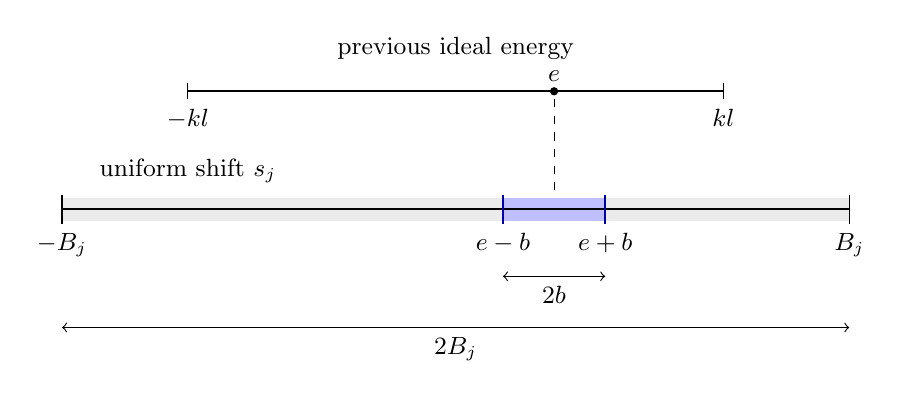
\begin{tikzpicture}[x=1cm,y=1cm,every node/.style={font=\small}]
 \node at (0,2.05) {previous ideal energy};
 \draw[thick] (-3.4,1.5)--(3.4,1.5);
 \draw (-3.4,1.4)--(-3.4,1.6) (3.4,1.4)--(3.4,1.6);
 \node[below] at (-3.4,1.4) {$-kl$};
 \node[below] at (3.4,1.4) {$kl$};
 \fill (1.25,1.5) circle (1.5pt);
 \node[above] at (1.25,1.5) {$e$};
 \draw[dashed] (1.25,1.4)--(1.25,.16);
 \fill[black!8] (-5,-.15) rectangle (5,.15);
 \fill[blue!25] (.6,-.15) rectangle (1.9,.15);
 \draw[thick] (-5,0)--(5,0);
 \draw (-5,-.18)--(-5,.18) (5,-.18)--(5,.18);
 \draw[blue!65!black,thick] (.6,-.18)--(.6,.18) (1.9,-.18)--(1.9,.18);
 \node[below] at (-5,-.18) {$-B_j$};
 \node[below] at (5,-.18) {$B_j$};
 \node[below] at (.6,-.18) {$e-b$};
 \node[below] at (1.9,-.18) {$e+b$};
 \node[above] at (-3.4,.22) {uniform shift $s_j$};
 \draw[<->] (.6,-.85)--(1.9,-.85);
 \node[below] at (1.25,-.85) {$2b$};
 \draw[<->] (-5,-1.5)--(5,-1.5);
 \node[below] at (0,-1.5) {$2B_j$};
\end{tikzpicture}
\caption{Capture at step $j=k+1$, shown schematically.
For an ideal spectral value $|e|\le kl$, the entire capture interval
$[e-b,e+b]$ lies in the sampling interval, giving probability
$2b/(2B_j)=b/B_j$. The actual propagated error has no assumed spectral
bound; for any of its spectral values the capture probability is at most
$b/B_j$.}
\label{fig:capture}
\end{figure}

For \eqref{eq:errorbound}, fix $t$ and all parameters from the previous
$k$ steps, so that $\zeta_k-\chi_k$ is fixed. No spectral support bound
on this error is available. For every real $e$,
\[
 \Pr_{s_j}(|e-s_j|\le b)
 =\frac{|[e-b,e+b]\cap[-B_j,B_j]|}{2B_j}\le\frac b{B_j}.
\]
The spectral theorem therefore gives the quadratic-form inequality
\[
 \frac1{2B_j}\int_{-B_j}^{B_j}
       \one_{\{|S_k-s|\le b\}}\,ds\le\frac b{B_j}\,1.
\]
Also $\Pr_{r_j}(|t-r_j|\le b)\le b/(2A)$ for every fixed $t$.
The two current sampling parameters are independent of each other and
of the past. The fresh vector has norm one, while $W_{-s_j}$ commutes
with $Q$ and does not affect its norm. Consequently
\[
 \E_{r_j,s_j}\|Q(v-v_0)\|^2
 \le a_j\|\zeta_k-\chi_k\|^2.
\]
Now integrate over $t$ and the past parameters to obtain
\[
 \E\|Q(v-v_0)\|^2\le a_j\E\|\zeta_k-\chi_k\|^2\le a_j\epsilon^2
\]
by \eqref{eq:idealclose}. Since $\|U_j-D_j\|\le2$, this proves the claim.

\paragraph{The contradiction.}
Since $Q$ commutes with the step operators,
$\|(U_j-D_j)v\|^2\ge\|(U_j-D_j)Qv\|^2$.
The triangle inequality in the mean-square Hilbert space, followed by
\eqref{eq:normloss}, shows that the expected squared-norm loss at step $j$
is at least
\begin{equation}\label{eq:positive-loss}
 \frac{a_j}{4}\left(\frac{\sqrt3}{2}c-2\epsilon\right)^2.
\end{equation}
The constant in parentheses is positive. On the other hand, inserting a
unit fresh vector and applying the outer shift do not change norm. The
losses therefore telescope from one and have total at most one. Since
$\sum_j a_j=\infty$, choosing sufficiently many steps contradicts
\eqref{eq:positive-loss}. Hence $U=D$.
\end{proof}
\section{The continuous core and the general inclusion}\label{sec:core}
The multiplication identity now determines the fixed points of the
bicentralizer flow in the core. We recall why the core fixed-point equality
yields an amenable subalgebra, then prove that equality in coordinates
adapted to $N$. The final reduction passes from factors to an arbitrary center and invokes the
existing amenable-subalgebra theorem.

\paragraph{The core criterion.}
For a type $\mathrm{III}_1$ bottom factor, the bicentralizer in the core
and its flow have the following description. Here
$\B(N\subset c(M),\varphi)$ uses the same asymptotic commutation condition
on bounded sequences in $N$, with the state $\varphi$ on $N$.
In the realization
$c(M)=M\rtimes_{\sigma^\varphi}\R$, with group unitaries $l(t)$, one has
\begin{equation}\label{eq:core-bic}
 \B(N\subset c(M),\varphi)=B\rtimes_{\sigma^\varphi}\R,
 \qquad \gamma_s(l(t))=e^{-its}l(t).
\end{equation}
The algebra identity is \cite[Proposition~7.2]{M1}; the action extends the
flow on $B$ as in \cite[Proposition~8.6, proof]{M1}.
One inclusion in the desired fixed-point equality is automatic:
\begin{equation}\label{eq:core-auto}
 N'\cap c(M)\subset\B(N\subset c(M),\varphi)^\gamma.
\end{equation}
This inclusion follows by combining \cite[Proposition~8.1 and its proof,
Theorem~6.20(5), and Proposition~8.4]{M1}. We will prove the reverse
inclusion. Equality is equivalent to the relative bicentralizer
conjecture by \cite[Proposition~8.6]{M1}.
For an expected inclusion, that conjecture is equivalent to the
\emph{weak Dixmier property} for $N\subset c(M)$:
\begin{equation}\label{eq:WD}
 \overline{\conv\{uxu^*:u\in\U(N)\}}^{\,w^*}
 \cap(N'\cap c(M))\ne\varnothing\qquad(x\in c(M)).
\end{equation}
With separable preduals, \eqref{eq:WD} is equivalent to the conclusion of
Theorem~\ref{thm:main}, by \cite[Theorem~D]{M1}.

\begin{proposition}\label{prop:corefixed}
If $N$ is a type $\mathrm{III}_1$ factor, then
\[
 \B(N\subset c(M),\varphi)^\gamma=N'\cap c(M).
\]
\end{proposition}
\begin{proof}
\leavevmode
\paragraph{The algebra generated by $N$ and $B$.}
By Theorem~\ref{thm:UD}, $L^*R=D$ is unitary. Since $L,R$ are isometries,
this implies $R=LD$, so their ranges agree. Put $A=B\vee N$.
The common range is $L^2(A,\varphi)$: it contains $\Omega$, is invariant
under left $N$ by its $R$ description and under left $B$ by its $L$
description, and is contained in $L^2(A,\varphi)$. Applying adjoints gives
invariance under the generated von Neumann algebra. Both $N$ and $B$ are
modularly invariant, so the expected algebra $A$ has a canonically embedded
core inside $c(M)$.

\paragraph{Coordinates adapted to $N$.}
Use $L$ to identify $L^2(A,\varphi)$ with $H\otimes K$. In these coordinates
left $B$ acts as $1\otimes B$, left $N$ acts as $D(N\otimes1)D^*$, and the
modular group is
\[
 e^{itX}\otimes\Delta_{\varphi|_B}^{it}.
\]
Represent $c(A)$ faithfully on $H\otimes K\otimes L^2(\R)$ with constant
base algebra and group unitaries
\[
 e^{itX}\otimes\Delta_{\varphi|_B}^{it}\otimes l_{\R}(t),
\]
where $l_\R$ is the translation representation. This is the usual regular
crossed-product representation after conjugating its variable base algebra
by the modular implementation.

Conjugate by $D^*$ on the first two positions. This removes the twist
from the action of $N$, which now acts on $H$ alone, and transfers it to
the core of $B$. Since $W_s$ commutes with $\Delta_{\varphi|_B}^{it}$, the algebra
$B\rtimes\R$ is represented, at spectral value $X=h$, by
\begin{equation}\label{eq:corefiber}
 a\longmapsto\gamma_{-h}(a)\otimes1,\qquad
 l(t)\longmapsto e^{ith}\Delta_{\varphi|_B}^{it}\otimes l_\R(t).
\end{equation}
The two transformations in \eqref{eq:corefiber} are the same flow:
on $B$ it is $\gamma_{-h}$, and on $l(t)$ it multiplies by $e^{ith}$.
Thus these fibers are a fixed normal representation of $B\rtimes\R$
composed with the core bicentralizer flow at $-h$, by \eqref{eq:core-bic}.
More explicitly, if $H=\int^\oplus H_h\,d\nu(h)$ and $\pi_0$ is the fixed
regular representation on $K\otimes L^2(\R)$, the representation of an
element $z\in B\rtimes\R$ is
\[
 \int^\oplus I_{H_h}\otimes\pi_0(\gamma_{-h}(z))\,d\nu(h).
\]
This normal direct-integral representation agrees with \eqref{eq:corefiber}
on generators, so the formula applies to the entire crossed product.

\paragraph{The fixed algebra.}
If $z$ is fixed by the core bicentralizer flow, then
$\pi_0(\gamma_{-h}(z))=\pi_0(z)$ in every fiber. It therefore acts on
$K\otimes L^2(\R)$ alone, while $N$ acts on $H$ alone. Hence it commutes
with $N$, proving
\[
 \B(N\subset c(M),\varphi)^\gamma\subset N'\cap c(M).
\]
The opposite inclusion is \eqref{eq:core-auto}, so the fixed algebras agree.
\end{proof}

\begin{proof}[Proof of Theorem~\ref{thm:main}]
\leavevmode
\paragraph{Factor bottom algebras.}
For a type $\mathrm{III}_1$ bottom factor,
Proposition~\ref{prop:corefixed} and \cite[Proposition~8.6 and Theorem~D]{M1}
give the weak Dixmier property \eqref{eq:WD}. The state on $N$ is a strictly
semifinite weight, as required there. For a bottom factor of any other type,
the same weak Dixmier property is \cite[Proposition~4.11]{M1}.
These factor cases allow arbitrary upper algebras.

\paragraph{Disintegration over the center.}
For a general $N$, put $J=\mathcal Z(N)$ and $M_0=J'\cap M$.
The passage to $M_0$ makes $J$ central in both algebras, so that we can
apply the factor cases fiber by fiber.
The modular action of $\varphi=\varphi\circ E_N$ fixes $J$ pointwise.
Consequently $M_0$ is modularly invariant, and $E_N$ restricts to a faithful
normal expectation $M_0\to N$. Moreover,
\begin{equation}\label{eq:center-core}
 J'\cap c(M)=c(M_0)
\end{equation}
inside the chosen core, by \cite[Proposition~4.7]{M1}.

Disintegrate $N\subset M_0$ over the common central algebra $J$, using the
probability measure $\mu$ determined by $\varphi|_J$.
The bottom fibers $N_z$ are factors because $J=\mathcal Z(N)$; the upper
fibers $(M_0)_z$ need not be factors. The simultaneous disintegration theorem
for operator-valued weights gives faithful normal fiber expectations
$E_z:(M_0)_z\to N_z$ and compatible faithful state fibers $\varphi_z$
\cite[Propositions~2.1--2.2 and Theorem~2.3]{IK2007}.
Indeed, $E_N$ is $J$-bimodular, and its fiber weights satisfy $E_z(1)=1$,
so they are conditional expectations. The state identity
$\varphi=\varphi\circ E_N$ and the modular actions also disintegrate,
as in the proof of that theorem.

To see the resulting core compatibility, write
$H_0=L^2(M_0,\varphi)=\int^\oplus H_z\,d\mu(z)$, where
$H_z=L^2((M_0)_z,\varphi_z)$. The regular representation of the core
on $L^2(\R,H_0)=\int^\oplus L^2(\R,H_z)\,d\mu(z)$ is given by
\[
 (\pi(a)\xi)(t)=\sigma_{-t}^\varphi(a)\xi(t),\qquad
 (l(s)\xi)(t)=\xi(t-s).
\]
Both formulas act fiberwise. A countable family of algebra generators and
the rational translation parameters generate the fiber cores; the common
central algebra $J$ is already present in the representation. Thus
$c(M_0)=\int^\oplus c((M_0)_z)\,d\mu(z)$ with the corresponding copies of
$N_z$. Separability supplies these standard measurable fields. The factor
cases and the direct-integral criterion \cite[Proposition~4.12]{M1} now give
the weak Dixmier property for $N\subset c(M_0)$.

\paragraph{Averaging into the central commutant.}
We have proved the weak Dixmier property inside $c(M_0)$. To apply it
to an arbitrary $x\in c(M)$, we first average $x$ into this smaller core.
The weak* compact convex hull of its orbit under
$\U(J)$ is preserved by the commuting affine maps $\Ad(u)$, $u\in\U(J)$.
The compact-convex fixed-point theorem for commuting affine maps gives a
common fixed point $y\in J'\cap c(M)=c(M_0)$. One can obtain it by taking
rectangular Ces\`aro averages for each finite family of commuting maps,
then using compactness and the finite-intersection property. Since $J\subset N$, this
point belongs to the weak* closed convex $N$-orbit hull of $x$.
That hull is $N$-invariant. Applying weak Dixmier averaging inside $c(M_0)$
therefore produces a point of $N'\cap c(M)$ still in the original hull.
This proves \eqref{eq:WD} for the original inclusion.

\paragraph{The amenable subalgebra.}
Finally \cite[Theorem~D, (3)$\Rightarrow$(4)]{M1} supplies an amenable
subalgebra $P\subset N$ with a faithful normal conditional expectation and
$P'\cap c(M)=N'\cap c(M)$. The expectation is faithful and normal by the
meaning of ``with expectation'' in that theorem. Unitality is automatic:
if $p=1_P<1_N$, bimodularity would imply $F(1-p)=0$, contradicting
faithfulness. This proves the result.
\end{proof}

\begin{thebibliography}{99}
\bibitem{AndoHaagerup2014}
H.~Ando and U.~Haagerup, \emph{Ultraproducts of von Neumann algebras},
J. Funct. Anal. \textbf{266} (2014), no.~12, 6842--6913.
\href{https://arxiv.org/abs/1212.5457v3}{arXiv:1212.5457v3}.

\bibitem{AHHM}
H.~Ando, U.~Haagerup, C.~Houdayer, and A.~Marrakchi,
\emph{Structure of bicentralizer algebras and inclusions of type III factors},
Math. Ann. \textbf{376} (2020), 1145--1194.
\href{https://arxiv.org/abs/1804.05706v2}{arXiv:1804.05706v2}.

\bibitem{Connes1982}
A.~Connes, \emph{Classification des facteurs}, in Operator Algebras and
Applications, Part 2 (Kingston, Ontario, 1980), Proc. Sympos. Pure Math.
\textbf{38}, American Mathematical Society, Providence, RI, 1982, 43--109.

\bibitem{Connes1985}
A.~Connes, \emph{Factors of type $\mathrm{III}_1$, property $L'_\lambda$,
and closure of inner automorphisms}, J. Operator Theory \textbf{14}
(1985), 189--211.

\bibitem{Haagerup}
U.~Haagerup, \emph{Connes' bicentralizer problem and uniqueness of the
injective factor of type $\mathrm{III}_1$}, Acta Math. \textbf{158} (1987),
95--148. \href{https://doi.org/10.1007/BF02392257}{doi:10.1007/BF02392257}.

\bibitem{HI2017}
C.~Houdayer and Y.~Isono, \emph{Unique prime factorization and bicentralizer
problem for a class of type III factors}, Adv. Math. \textbf{305}
(2017), 402--455.
\href{https://arxiv.org/abs/1503.01388v3}{arXiv:1503.01388v3}.

\bibitem{HoudayerMarrakchi2026}
C.~Houdayer and A.~Marrakchi, \emph{The classification of flows on
$\mathrm{II}_1$ factors and Connes' bicentralizer problem}, 2026,
version 1, September 10, 2026.
\href{https://arxiv.org/abs/2609.11462v1}{arXiv:2609.11462v1}.

\bibitem{IK2007}
R.~Ichihara and S.~Kawakami, \emph{Disintegration of operator valued
weights}, Scientiae Mathematicae Japonicae Online \textbf{e-2007}
(2007), 693--699.
\href{https://www.jams.jp/scm/contents/e-2007-7/2007-63.pdf}{Publisher PDF}.

\bibitem{M0}
A.~Marrakchi, \emph{Full factors, bicentralizer flow and approximately inner
automorphisms}, Invent. Math. \textbf{222} (2020), 375--398.
\href{https://arxiv.org/abs/1811.10253v2}{arXiv:1811.10253v2}.

\bibitem{M1}
A.~Marrakchi, \emph{Kadison's problem for type III subfactors and the
bicentralizer conjecture}, Invent. Math. \textbf{239} (2025), 79--163.
\href{https://arxiv.org/abs/2308.15163v3}{arXiv:2308.15163v3}.

\bibitem{M2}
A.~Marrakchi, \emph{Kadison's problem and ergodicity of the bicentralizer flow},
2026, version 2, 11 August 2026.
\href{https://arxiv.org/abs/2606.23636v2}{arXiv:2606.23636v2}.

\bibitem{MarrakchiVaes2024}
A.~Marrakchi and S.~Vaes, \emph{Ergodic states on type $\mathrm{III}_1$
factors and ergodic actions}, J. Reine Angew. Math. \textbf{809}
(2024), 247--260.
\href{https://arxiv.org/abs/2305.14217v3}{arXiv:2305.14217v3}.

\bibitem{Masuda2005}
T.~Masuda, \emph{An analogue of Connes--Haagerup approach for classification
of subfactors of type $\mathrm{III}_1$}, J. Math. Soc. Japan \textbf{57}
(2005), 959--1001.
\href{https://doi.org/10.2969/jmsj/1150287301}{doi:10.2969/jmsj/1150287301}.

\bibitem{BoundedRecovery}
OpenAI, \emph{Bounded recovery for modular spectral averages},
OpenAI Math Release preprint
\href{https://github.com/openai/math/blob/main/preprints/Bounded-recovery-for-modular-spectral-averages-September-23-2026/Bounded-recovery-for-modular-spectral-averages-September-23-2026.pdf}{OAI:Bounded-recovery-for-modular-spectral-averages-September-23-2026},
2026.

\bibitem{Popa1981}
S.~Popa, \emph{On a problem of R.~V.~Kadison on maximal abelian
$*$-subalgebras in factors}, Invent. Math. \textbf{65} (1981), 269--281.
\href{https://doi.org/10.1007/BF01389015}{doi:10.1007/BF01389015}.

\bibitem{Takesaki1972}
M.~Takesaki, \emph{Conditional expectations in von Neumann algebras},
J. Funct. Anal. \textbf{9} (1972), 306--321.
\href{https://doi.org/10.1016/0022-1236(72)90004-3}{doi:10.1016/0022-1236(72)90004-3}.

\bibitem{Takesaki2003}
M.~Takesaki, \emph{Theory of Operator Algebras II}, Encyclopaedia of
Mathematical Sciences \textbf{125}, Springer-Verlag, Berlin, 2003.
\href{https://doi.org/10.1007/978-3-662-10451-4}{doi:10.1007/978-3-662-10451-4}.

\end{thebibliography}
\end{document}
